\documentclass[main.tex]{subfiles}

\begin{document}
\section{PCT Project
}
\textit{This chapter will go over the PCT-project that is currently under development by the Department of Physics and technology in Bergen. It will discuss the DTC being developed for the project, how it tracks and measures the energy protons. Then a technical overview of the system is given, along with how the PCS and the control software of this thesis will be implemented.}

The Bergen \gls{pct}-project is a collaboration with the University of Bergen and many other universities and other institutions in the world, to build a \gls{pct}-scanner to be used in proton treatment. The design is based on using a \acrfull{dtc} to detect protons emitted from the particle accelerator. In particular, the focus is on creating a scanner for use on pediatric patients. This is due to pediatric patients suffer more from long term side effects of \gls{rt} and therefore proton therapy is a more suitable treatment.


\subsection{ALPIDE chips}

The basic pixel detector sensor used for this project is the \gls{alpide}-chips that were designed for the upgrade of the \gls{its} during the long shutdown of the \gls{lhc} during the 2019-2020 period. The chips is categorized as \gls{maps} with a span of 1.5 cm x 3 cm. The sensor is made out of a matrix of 512 x 1024 pixels and they function as binary hit/no hit sensors. A detection threshold is set for the chip, suppressing all hits that are below the threshold level, functioning as data compression for non-relevant data, such as from noise and radiation. A cross section of the \gls{alpide} sillcon is shown in \autoref{fig: alpide_cross}.

\begin{figure}[!htpb]
    \centering
    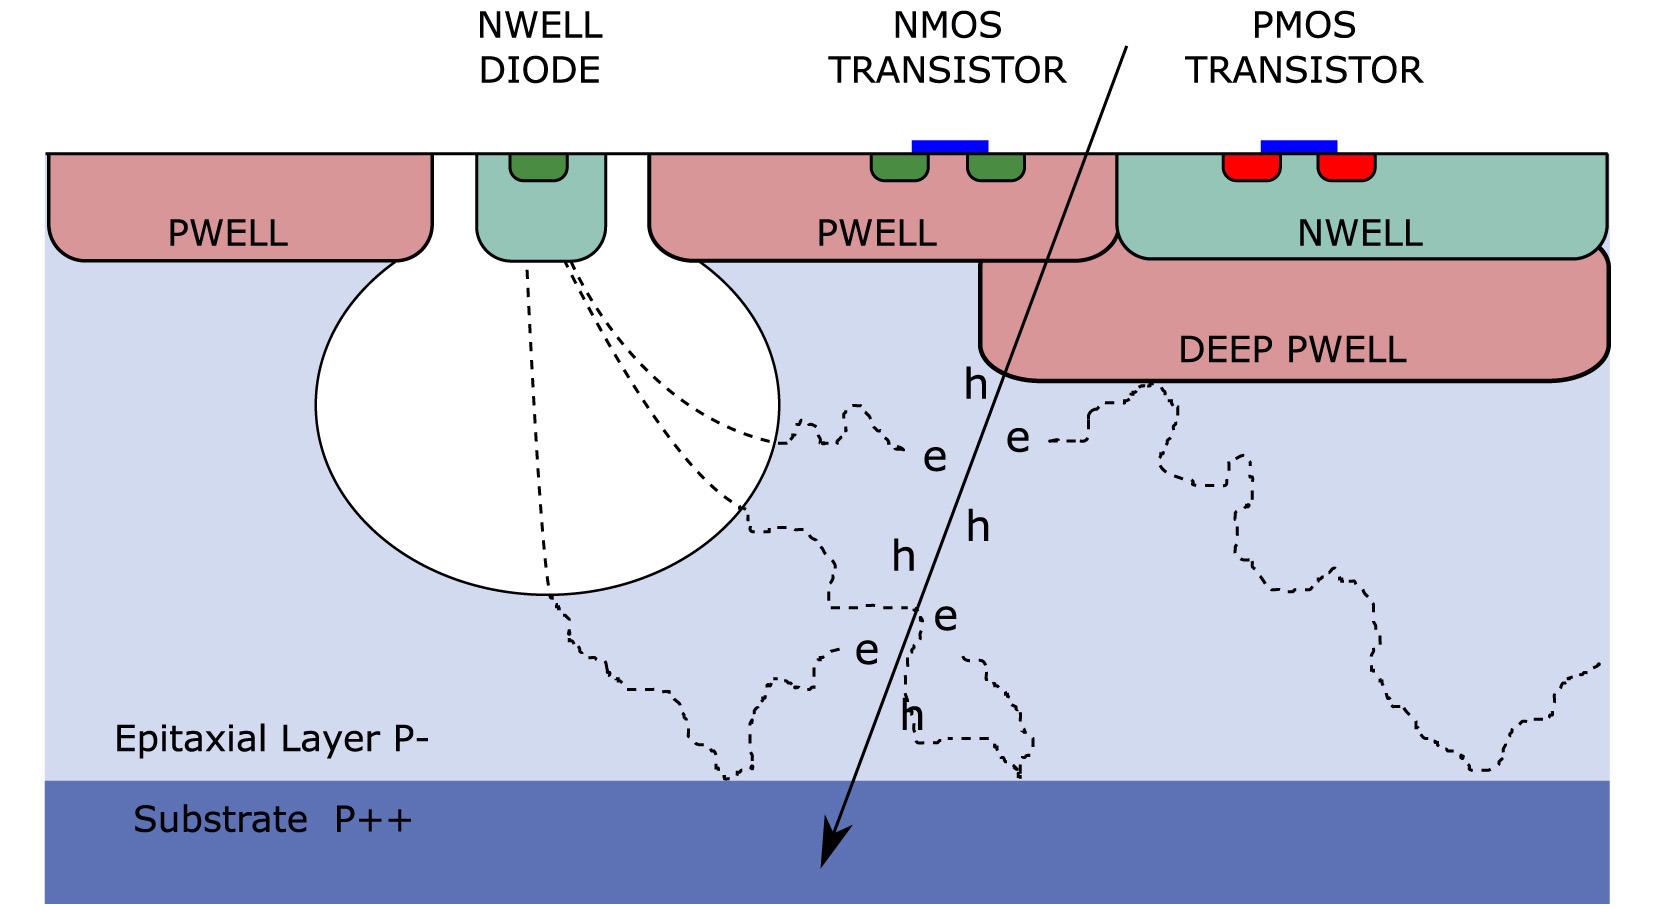
\includegraphics[width=12cm]{images/alpide_chip.jpg}
    \caption{Cross section of an ALPIDE-chip, showing a particle entering the silicon and causes a hit ot register.}
    \label{fig: alpide_cross}
\end{figure}
\FloatBarrier


The figure shows a particle entering the silicon and releasing electron-hole pairs from the Epitaxial layer. The charge moves to the depletion region around the collection diode and if it reaches the set threshold, registers a hit on the pixel.

In the \gls{pct} project, nine \gls{alpide}-chips are bonded together on one flex cable, which is defined as one "string". A \gls{alpide} string is shown in \autoref{fig: alpide_physical}.

\begin{figure}[!htpb]
    \centering
    \includegraphics[width=12cm]{images/alpideStringPhysical.png}
    \caption{Image of a string, highlighting the ALPIDE chip, chip cable, and flex cable.}
    \label{fig: alpide_physical}
\end{figure}
\FloatBarrier

From the figure we can see that half of the string is covered by the chip itself, and the other half is the flex cable the chips are mounted to.

\subsection{DTC}

The \gls{dtc} is distinct in that it combines proton tracking and energy measurement into one technology. It is made out of 43 layers of pixel detectors, where 2 layers in the rear is used to track the trajectory of the protons and the other 41 measures their energy. A model of it is given in \autoref{fig: DTC_image}.

\begin{figure}[!ht]
    \centering
    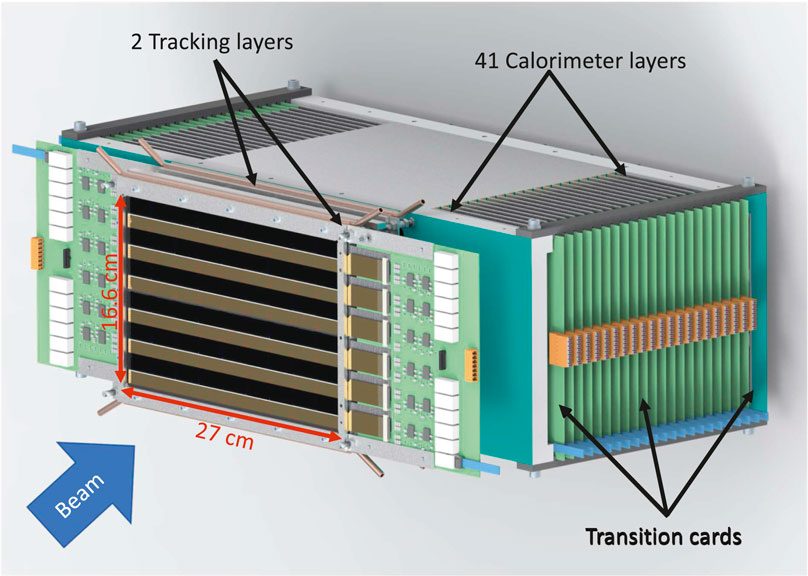
\includegraphics[scale = 0.5]{images/dtc.jpg}
    \caption{Model of DTC used in the pCT project. Dimensions of the tracker are (27 cm x 16.6 cm).}
    \label{fig: DTC_image}
\end{figure}
\FloatBarrier

A \gls{dtc} is usually realized with front and rear trackers, but only the rear trackers are used in this prototype. Studies have shown that single-sided proton imaging using \gls{pbs} can lead to similar spatial resolution in the image as compared to double-sided\cite{pbs_result}. the single-sided tracker also comes with a few advantages, such as lower material budget and less complexity in the rigging of the \gls{dtc}.

The layers of \gls{dtc} are functionally identical, but the calorimeter layers are made with aluminum absorbers to fully contain the energy range from the proton beam, which is estimated to be 230 MeV. The tracking layer must have minimum material budget to minimize the scattering of the protons, which can affect the accuracy of the image. The tracking layers are used to track the angle the protons exit the patient, the two layers provides the linear path of the proton and the angle is derived from that. Based on the angle, one can make an estimate of the most likely path taken by the protons as it was moving through the patient. This data is crucial for reconstructing the CT-image.

A layer of the \gls{dtc} is realized using 12 strings of \gls{alpide}-chips. a layer is made out of two half layers, and a half layer is made out of two "slabs of \gls{alpide}-chips. the "slabs" are three strings glued together, a picture of a half layer is shown in \autoref{fig: half_layer}.

\begin{figure}[!ht]
    \centering
    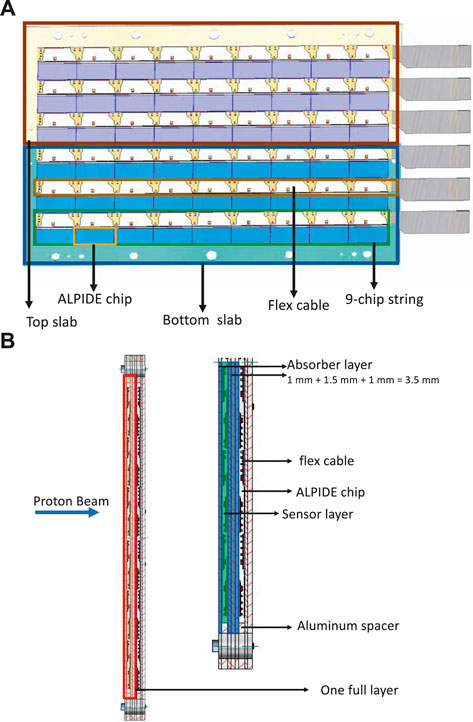
\includegraphics[scale = 0.5]{images/half_layer.jpg}
    \caption{A) Image of half layer, highlighting the various components of the layer. B) side view of a half layer and a full layer\cite{pct_project}}
    \label{fig: half_layer}
\end{figure}
\FloatBarrier

We can note from the figure that the \gls{alpide}-chip only covers about half of the layer, the rest of the space is dedicated to the flex cable. Two half layers are stacked in such a way that the \gls{alpide}chips of one half layer covers the flex cable of the other, ensuring full area coverage, giving us a full layer of the \gls{dtc}.

\subsection{Detector Control System}

The \gls{dcs} of the \gls{dtc} is still in development. The \gls{dcs} is made of two parts: readout and power delivery. The readout electronics retrieve the pixel hit data from the \gls{alpide}s, while the power delivery is responsible for delivering power to the strings and monitor their current consumption. A block diagram showing the concept for the \gls{dcs} is shown in \autoref{fig: dcs_concept}

\begin{figure}[!ht]
    \centering
    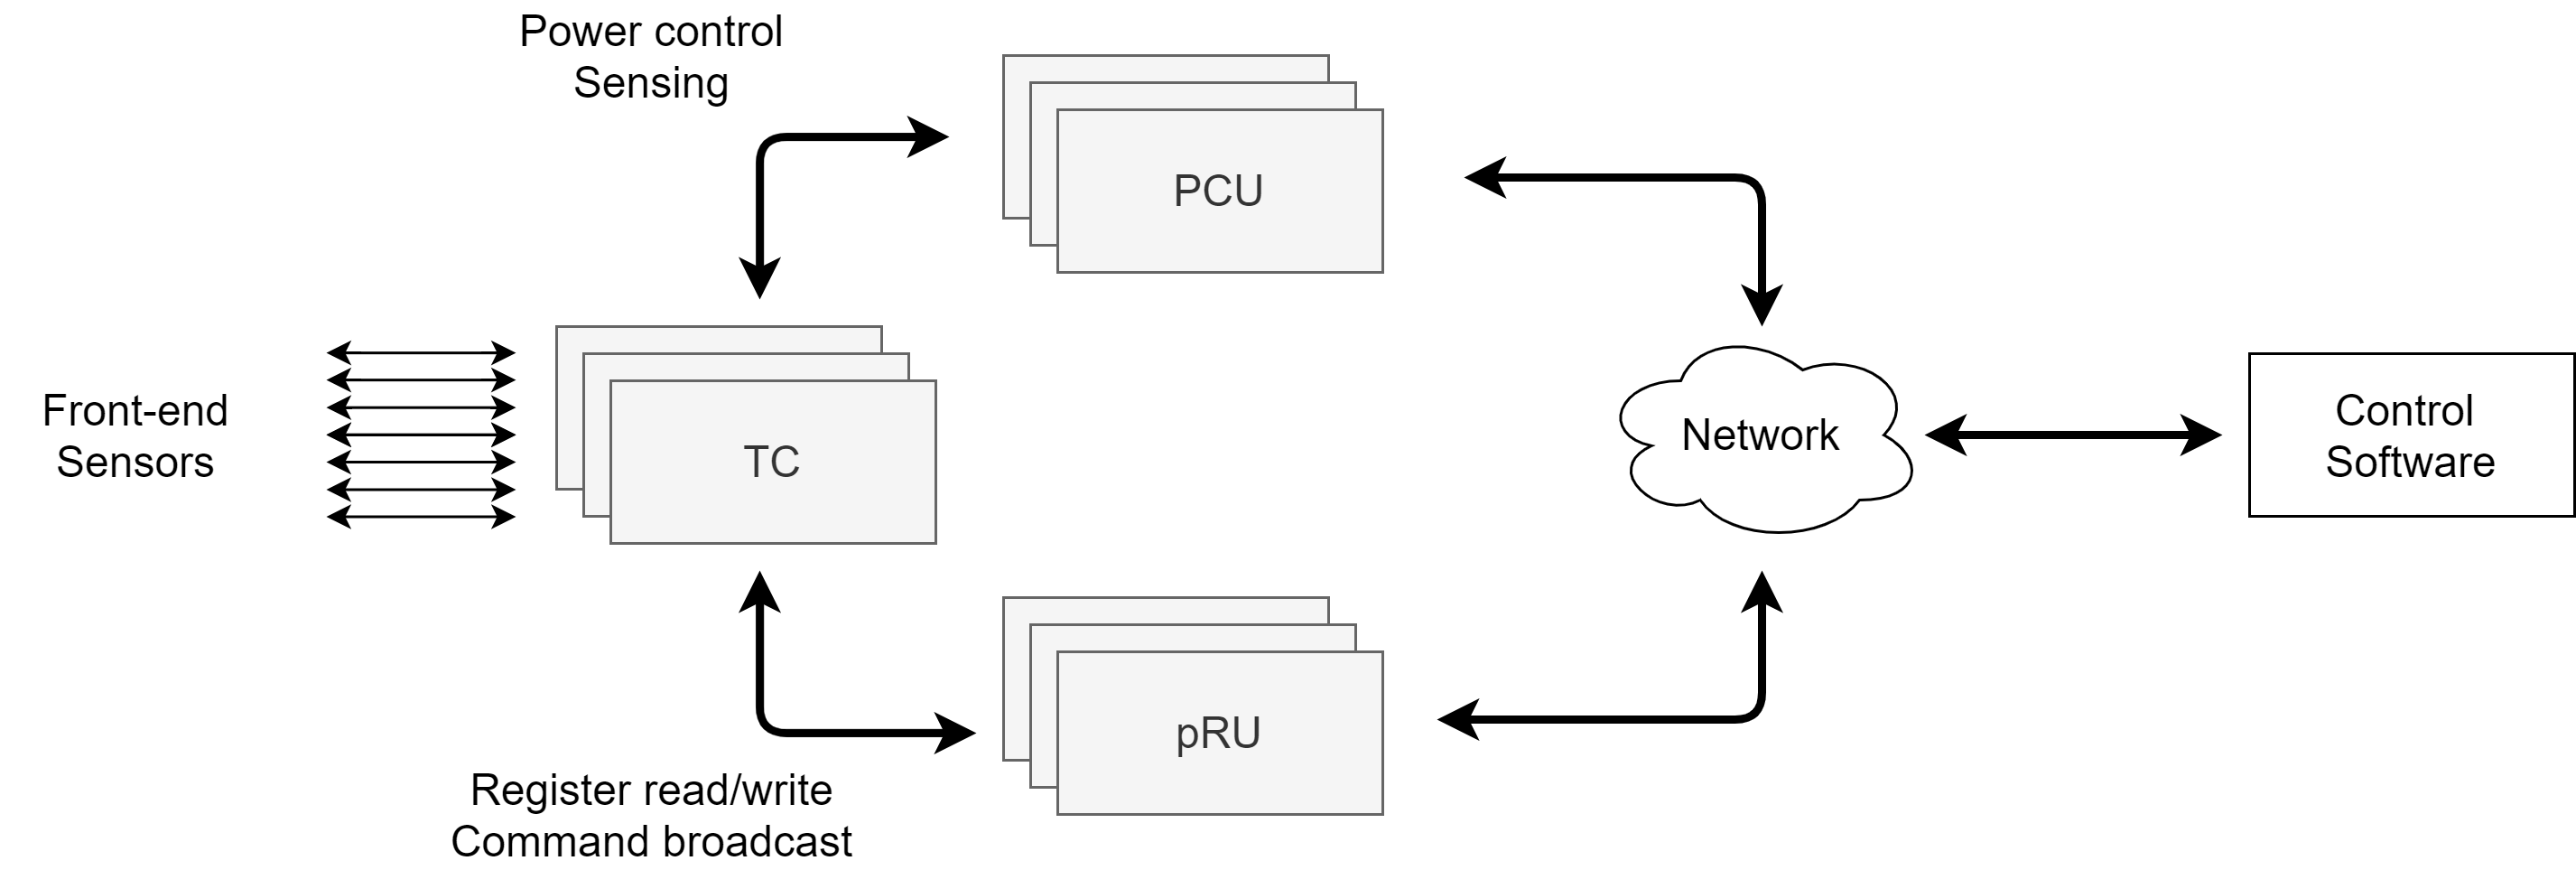
\includegraphics[width=15cm]{images/dcs_concept.png}
    \caption{Block diagram showing the general concept of the DCS.}
    \label{fig: dcs_concept}
\end{figure}
\FloatBarrier

Control software sends and retrieves data to the power delivery system and readout unit through a network, and the units relays power and data to the \gls{tc} that is connected to the sensors. The "Network" is the connection between the units and the control software, Ethernet cables are used for communication and IPbus communication protocol is used to establish an interface. The IPbus interface is built using an \gls{fpga} and as such, each unit uses its own \gls{fpga} to handle communication. The current implementation of these two systems is shown in \autoref{fig: dcs_diagram}

\begin{figure}[!ht]
    \centering
    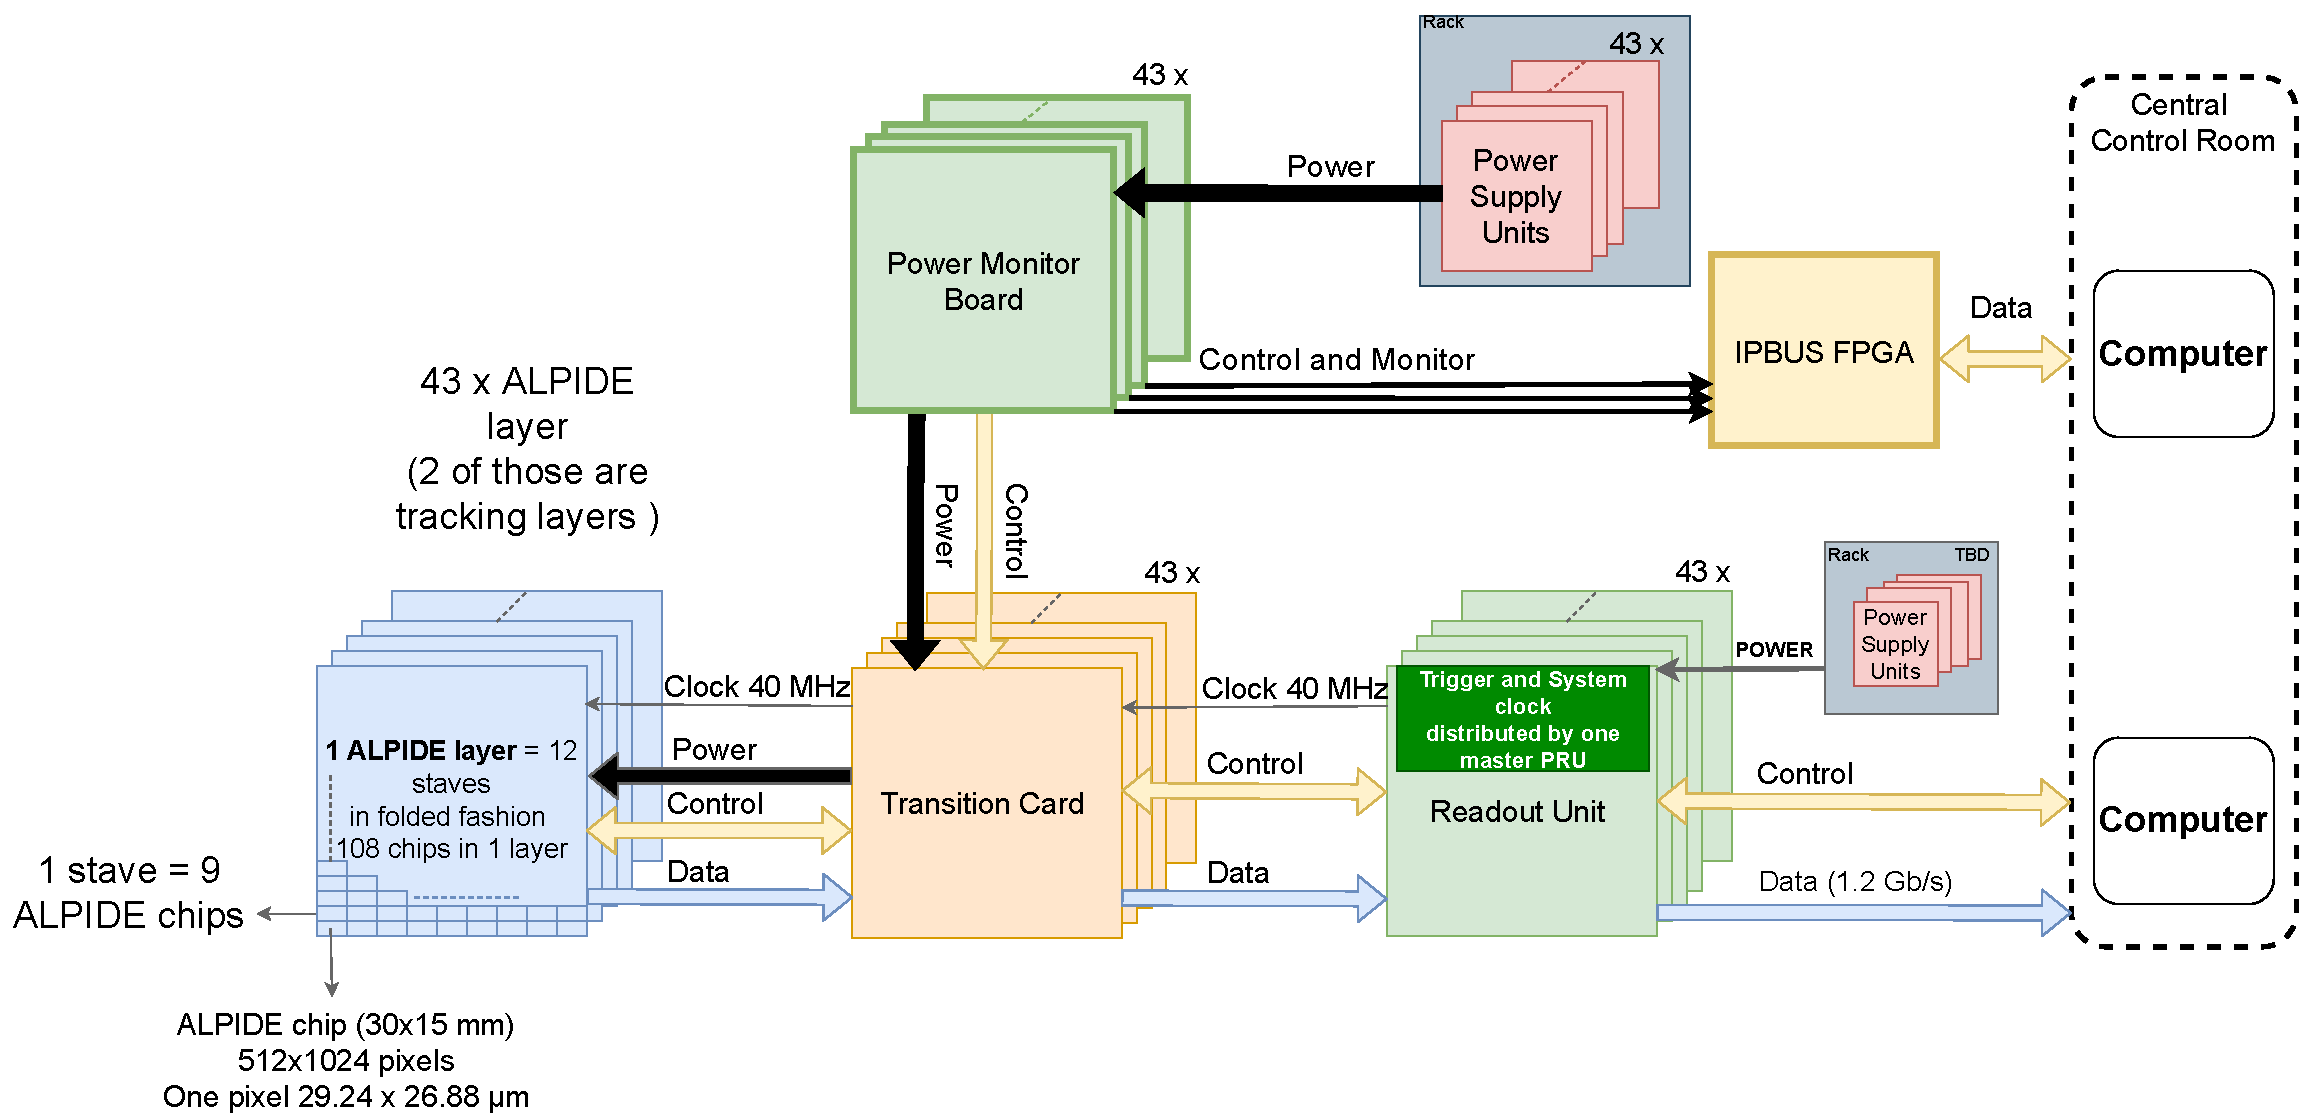
\includegraphics[scale=0.4]{images/pCT_Current_layout-CurrentSystemOverview.pdf}
    \caption{Block diagram of the current design of the DCS. The upper part shows the power delivery and monitoring system, and lower half is the readout unit.}
    \label{fig: dcs_diagram}
\end{figure}
\FloatBarrier

From the upper half of \autoref{fig: dcs_diagram}, the power delivery system is realized with 43 monitor boards, delivering power to the \gls{tc}s, and monitor of these boards are handled by an \gls{fpga} that is connected to the control software.

In a similar manner the bottom half of the figure showcases the 43 readout units in charge of sending and retrieving data to and from the \gls{alpide}-chips. The readout units along with control software in the control room encompasses the control system for the readout electronics. The \gls{mb} and readout units will be connected to the \gls{tc}s through 3 metres of Firefly-cables 

Another aspect to be considered in the \gls{dcs} is the radiation the various components are exposed to. The radiation from the proton therapy can have an adverse effect on circuitry and hardware. From \autoref{fig: dcs_diagram}, it is estimated that the \gls{tc} will be in the high radiation zone due to having to be close to the actual sensors, while the readout units and \gls{mb} will have minimal exposure to radiation, due to being separated by 3 metres of Firefly cables. This means that it is not necessary to accommodate more than the usual radiation protection for components involved in the power control and readout systems.


\subsection{Control Systems}

Readout units and power supply board both require a software end point that essentially controls the entire system. This entails creating a system that can setup and configure the various parts of the system and also monitoring the system and report errors, i.e. we need to create a monitoring and configuration system.

A control system generally is made out of sensors, a controller to control and retrieve data from the sensors, a supervisory computer that manages the process for the sensors, and \gls{hmi} software. The \gls{hmi} software provides access to the data from the sensors to the user and if needed, also allow the user to modify and processes in the system.


\subsubsection{SCADA systems}
There are various control systems that have been made over the years in industries such as oil and gas, chemical manufacturing and fabrication. The most common type of control systems in industrial settings is \gls{scada}. \gls{scada} systems have four main functions: data collection, network data communication, data presentation, and remote monitoring and supervisory control\cite{scada_intro}. Although today, many control systems is based on \gls{iot}, which has a similar architecture, but \gls{iot} bases itself on utilizing cloud-networking and processing for its communication infrastructure. Due to lack of wireless communication in the \gls{pct}-project, focus will be on how \gls{scada} systems are developed and what that means for the project.

A \gls{scada} system typically is made out of five components:

\begin{itemize}
    \item Field devices and signals
    \item \acrfull{ppc}
    \item \acrfull{hmi}
    \item Database servers
    \item Communication infrastructure
\end{itemize}

Field devices and signals encompasses all sensors and the actuators that controls them. For \gls{pct}, this includes the \gls{alpide}-chips, temperature and power measurement, and cooling. \gls{ppc} is responsible for automatically controlling the field devices, as well as retrieving data from them and send it to the \gls{hmi}. \gls{hmi} is the software being executed on the main computer and is made of a user interface and database manager. The database server usually contains configuration and monitoring data from the field devices, and the communication infrastructure used in \gls{scada} systems is usually ethernet based.

\subsubsection{Communication network}
There are various communication networks that can be used in a \gls{scada}-system, since all data from the sensors in the \gls{pct} project comes from IPbus, it makes sense for one master computer to receive the data from the IPbus and process it, or send to other computers for processing. (McCrady, 2013) describes in his book of such a communication topology\cite{scada_design}. An example of a \textit{star} topology is shown in \autoref{fig: scada_star}.

\begin{figure}[!ht]
    \centering
    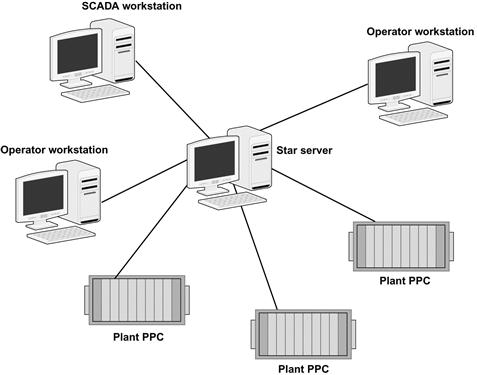
\includegraphics[scale=0.6]{images/scada_topology.png}
    \caption{Example of a star topology communication infrastructure used for SCADA systems\cite{scada_design}}
    \label{fig: scada_star}
\end{figure}
\FloatBarrier

In the \gls{pct}-project, the main computer can be connected to readout, power delivery, and cooling, leading to a \textit{star} topology, even if no other computers are connected.

\subsubsection{I/O Signals}

Important in a \gls{scada} system is to identify all signals to be used and retrieved by the field devices. Knowing all signals to be used in a system will give us an estimate of the requirements of the system as well as aid in the development process.

Power delivery uses a microcontroller to manage power output as well as temperature of the sensors. The microcontroller measures analog voltage(AVDD), digital voltage(DVDD), PWELL voltage, and the temperature of strings. It also have two register for each measurement that dictates the threshold levels, which will make the microcontroller turn off the power if these levels are exceeded. if we include monitoring an error register, and configuring enable signals for the strings, it will then result in 8 input/configuration signals and 8 output/monitoring signals.

\notinmain{Skriv meir om readout og cooling I/O signaler her, ha med ein tabell og kanskje}

\subsubsection{Software documentation}
Another important aspect of such a control system is having a consistent programming standard and complete software documentation. \gls{scada} and similar systems often have a long shelf time, and a well documented system will make maintenance and work in the future be much easier. In general, starting with good software documentation and expanding upon it during the project development will lead to sufficient documentation of the entire system.

A consistent programming standard helps in debugging and in expanding functionality of the system. \gls{oop} is a very common programming paradigm that is used to give structure to programs and increase reusability and maintainability of the code. Systems designed to manage large data acquisition, such as a \gls{pet}-scan system, have in the past used \gls{oop} to design and manage large programs\cite{pet_control_system}, this suggest that this programming structure is viable for the design of the control system in the \gls{pct}-project.

\end{document}